\section{泡利矩阵}

\begin{quotation}
``在科学中摧毁一个老的结构比建立一个持久的新结构容易。''\qquad 戴森
\end{quotation}


\begin{figure}[h]
\begin{center}
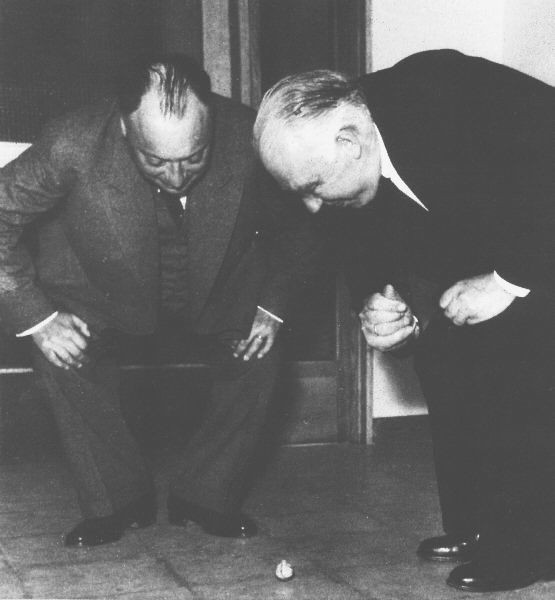
\includegraphics[clip,width=6cm]{Spin/bohrandpauli.jpg}
\caption{玻尔和泡利在玩陀螺}
\end{center}
\end{figure}


由于电子自旋无经典对应物,所以无法直接把电子自旋算符(自旋$1/2$算符)表示为$\left( {\widehat r,\widehat p} \right)$的函数。为求出电子自旋算符的正确表示,首先总结电子自旋的性质:


\begin{enumerate}
    \item 自旋具有角动量的特征,所以自旋算符应满足角动量算符的对易关系:

\begin{equation}\label{28-3}
\widehat{\mathord{\buildrel{\lower3pt\hbox{$\scriptscriptstyle\rightharpoonup$}}
\over S} } \times \widehat{\mathord{\buildrel{\lower3pt\hbox{$\scriptscriptstyle\rightharpoonup$}}
\over S} } = i\hbar \widehat{\mathord{\buildrel{\lower3pt\hbox{$\scriptscriptstyle\rightharpoonup$}}
\over S} }
\end{equation}


    \item $\vec S$在$z$方向取值只能为$ \pm {\textstyle{\hbar  \over 2}}$, $\hat S_z$的本征值是$ \pm {\textstyle{\hbar  \over 2}}$: $s_z  =  \pm {\textstyle{\hbar  \over 2}}$

同理:$\hat S_y$、$\hat S_z$的本征值也是$ \pm {\textstyle{\hbar  \over 2}}$: $s_z  =  \pm {\textstyle{\hbar  \over 2}}$,即:$s_x^2  = s_y^2  = s_z^2  = \frac{{\hbar ^2 }}{4}$


所以$\hat S^2$的本征值为:$S^2  = s\left( {s + 1} \right)\hbar ^2  = S_x^2  + S_y^2  + S_z^2  = {\textstyle{3 \over 2}}\hbar ^2 $
   \end{enumerate}


只要满足上述(1)(2)性质,就是电子自旋算符(自旋$1/2$算符)的正确表示;
显然对电子自旋算符的表示可以有很多种。本节我们将介绍自旋$1/2$算符的泡利矩阵表示。


\subsection{电子自旋的泡利矩阵表示}

引入算符$\hat \sigma$: $\widehat S = \frac{\hbar }{2}\widehat\sigma $,即:

\begin{equation}\label{28-4}
\widehat S_x  = \frac{\hbar }{2}\widehat\sigma _x , \widehat S_y  = \frac{\hbar }{2}\widehat\sigma _y, \widehat S_z  = \frac{\hbar }{2}\widehat\sigma _z
\end{equation}

为满足对易关系~\ref{28-3},得到$\hat \sigma$满足的对易关系:$\widehat\sigma  \times \widehat\sigma  = 2i\widehat\sigma $,即:


\begin{equation}\label{28-5}
\left\{ \begin{array}{l}
 \widehat\sigma _x \widehat\sigma _y  - \widehat\sigma _y \widehat\sigma _x  = 2i\widehat\sigma _z  \\
 \widehat\sigma _y \widehat\sigma _z  - \widehat\sigma _z \widehat\sigma _y  = 2i\widehat\sigma _x  \\
 \widehat\sigma _z \widehat\sigma _x  - \widehat\sigma _x \widehat\sigma _z  = 2i\widehat\sigma _y  \\
 \end{array} \right.
\end{equation}


$\hat S_z$的本征值是$ \pm {\textstyle{\hbar  \over 2}}$,所以:$\sigma_z$的本征值为$ \pm 1$;同理:$\sigma_x$、$\sigma_y$的本征值为$\pm 1$。

所以:$\sigma _x^2  = \sigma _y^2  = \sigma _z^2  = 1$

所以:$\widehat\sigma _x \widehat\sigma _y  + \widehat\sigma _y \widehat\sigma _x  = \frac{1}{{2i}}\left( {\widehat\sigma _y \widehat\sigma _z  - \widehat\sigma _z \widehat\sigma _y } \right)\widehat\sigma _y  + \frac{1}{{2i}}\widehat\sigma _y \left( {\widehat\sigma _y \widehat\sigma _z  - \widehat\sigma _z \widehat\sigma _y } \right) = 0$


同理:$\widehat\sigma _y \widehat\sigma _z  + \widehat\sigma _z \widehat\sigma _y  = \widehat\sigma _z \widehat\sigma _x  + \widehat\sigma _x \widehat\sigma _z  = 0$(反对易关系)

在$\hat \sigma_z$表象中求解,$\sigma_z$的本征值为$\pm 1$,所以$\hat \sigma_z$在自身表象中为对角矩阵,矩阵元为本征值:

$\widehat\sigma _z  = \left( {\begin{array}{*{20}c}
   1 & 0  \\
   0 & { - 1}  \\
\end{array}} \right)$
,$\widehat\sigma _z ^2  = \left( {\begin{array}{*{20}c}
   1 & 0  \\
   0 & 1  \\
\end{array}} \right) = 1$

为求得$\hat \sigma_x$和$\hat \sigma_y$在$\hat \sigma_z$表象中的矩阵表示,设:


$\widehat\sigma _x  = \left( {\begin{array}{*{20}c}
   {a_{11} } & {a_{12} }  \\
   {a_{21} } & {a_{22} }  \\
\end{array}} \right)$
,$\widehat\sigma _y  = \left( {\begin{array}{*{20}c}
   {b_{11} } & {b_{12} }  \\
   {b_{21} } & {b_{22} }  \\
\end{array}} \right)$

利用反对易关系:

$\begin{array}{l}
 \widehat\sigma _z \widehat\sigma _x  + \widehat\sigma _x \widehat\sigma _z  = \left( {\begin{array}{*{20}c}
   1 & 0  \\
   0 & { - 1}  \\
\end{array}} \right)\left( {\begin{array}{*{20}c}
   {a_{11} } & {a_{12} }  \\
   {a_{21} } & {a_{22} }  \\
\end{array}} \right) + \left( {\begin{array}{*{20}c}
   {a_{11} } & {a_{12} }  \\
   {a_{21} } & {a_{22} }  \\
\end{array}} \right)\left( {\begin{array}{*{20}c}
   1 & 0  \\
   0 & { - 1}  \\
\end{array}} \right) \\
  = \left( {\begin{array}{*{20}c}
   {a_{11} } & {a_{12} }  \\
   { - a_{21} } & { - a_{22} }  \\
\end{array}} \right) + \left( {\begin{array}{*{20}c}
   {a_{11} } & { - a_{12} }  \\
   {a_{21} } & { - a_{22} }  \\
\end{array}} \right) = 2\left( {\begin{array}{*{20}c}
   {a_{11} } & 0  \\
   0 & { - a_{22} }  \\
\end{array}} \right) = 0 \\
 \end{array}$

所以:$a_{11}  = a_{22}  = 0$,即:$\widehat\sigma _x  = \left( {\begin{array}{*{20}c}
   0 & {a_{12} }  \\
   {a_{21} } & 0  \\
\end{array}} \right)$


$\widehat\sigma _x^2  = \left( {\begin{array}{*{20}c}
   0 & {a_{12} }  \\
   {a_{21} } & 0  \\
\end{array}} \right)\left( {\begin{array}{*{20}c}
   0 & {a_{21}^* }  \\
   {a_{12}^* } & 0  \\
\end{array}} \right) = \left( {\begin{array}{*{20}c}
   {\left| {a_{12} } \right|^2 } & 0  \\
   0 & {\left| {a_{21} } \right|^2 }  \\
\end{array}} \right) = \left( {\begin{array}{*{20}c}
   1 & 0  \\
   0 & 1  \\
\end{array}} \right)$

所以:$\left| {a_{12} } \right|^2  = \left| {a_{21} } \right|^2  = 1$



由矩阵的厄密性:$a_{12}  = a_{21}^* $,即:$a_{21} a_{21}^*  = a_{21} a_{12}  = 1$


假设:$a_{12}  = e^{i\alpha } $,$\alpha$为实数;$a_{21}  = e^{ - i\alpha } $


即:$\widehat\sigma _x  = \left( {\begin{array}{*{20}c}
   0 & {e^{i\alpha } }  \\
   {e^{ - i\alpha } } & 0  \\
\end{array}} \right)$,不失一般性,假设$\alpha = 0$,则:$\widehat\sigma _x  = \left( {\begin{array}{*{20}c}
   0 & 1  \\
   1 & 0  \\
\end{array}} \right)$


利用:$\widehat\sigma _y  = \frac{1}{{2i}}\left( {\widehat\sigma _z \widehat\sigma _x  - \widehat\sigma _x \widehat\sigma _z } \right)$

$\begin{array}{l}
 \widehat\sigma _y   = \frac{1}{{2i}}\left\{ {\left( {\begin{array}{*{20}c}
   1 & 0  \\
   0 & { - 1}  \\
\end{array}} \right)\left( {\begin{array}{*{20}c}
   0 & 1  \\
   1 & 0  \\
\end{array}} \right) - \left( {\begin{array}{*{20}c}
   0 & 1  \\
   1 & 0  \\
\end{array}} \right)\left( {\begin{array}{*{20}c}
   1 & 0  \\
   0 & { - 1}  \\
\end{array}} \right)} \right\} \\
  = \frac{1}{{2i}}\left\{ {\left( {\begin{array}{*{20}c}
   0 & 1  \\
   { - 1} & 0  \\
\end{array}} \right) - \left( {\begin{array}{*{20}c}
   0 & { - 1}  \\
   1 & 0  \\
\end{array}} \right)} \right\} = \frac{1}{{2i}}\left( {\begin{array}{*{20}c}
   0 & 2  \\
   { - 2} & 0  \\
\end{array}} \right) = \left( {\begin{array}{*{20}c}
   0 & { - i}  \\
   i & 0  \\
\end{array}} \right) \\
 \end{array}$


于是得到$\hat \sigma_z$表象中的泡利矩阵:

\begin{equation}\label{pauli matrix}
\widehat\sigma _x  = \left( {\begin{array}{*{20}c}
   0 & 1  \\
   1 & 0  \\
\end{array}} \right)
,
\widehat\sigma _y  = \left( {\begin{array}{*{20}c}
   0 & { - i}  \\
   i & 0  \\
\end{array}} \right),
\widehat\sigma _z  = \left( {\begin{array}{*{20}c}
   1 & 0  \\
   0 & { - 1}  \\
\end{array}} \right)
\end{equation}


这三个矩阵与单位矩阵$1 = \left( {\begin{array}{*{20}c}
   1 & 0  \\
   0 & 1  \\
\end{array}} \right)$一同构成一组正交完备归一基,可用来描述仅有有两种状态的物理量。

\index{Pauli Matrix: 泡利矩阵}

\subsection{含自旋的波函数}


考虑自旋后电子波函数:$\psi \left( {r,t,s_z } \right)$,由于$s_z  =  \pm {\textstyle{1 \over 2}}\hbar $只有两种取值,所以波函数可写为两分量的形式:$\psi _1  = \psi \left( {r,t,{\textstyle{\hbar  \over 2}}} \right)$,$\psi _2  = \psi \left( {r,t, - {\textstyle{\hbar  \over 2}}} \right)$



写为矩阵形式:


\begin{equation}\label{28-6-1}
\Psi  = \left( {\begin{array}{*{20}c}
   {\psi _1 }  \\
   {\psi _2 }  \\
\end{array}} \right) = \psi _1 \left( {\begin{array}{*{20}c}
   1  \\
   0  \\
\end{array}} \right) + \psi _2 \left( {\begin{array}{*{20}c}
   0  \\
   1  \\
\end{array}} \right)
\end{equation}

定义自旋波函数:$\chi _ +   = \left( {\begin{array}{*{20}c}
   1  \\
   0  \\
\end{array}} \right)$,$\chi _ -   = \left( {\begin{array}{*{20}c}
   0  \\
   1  \\
\end{array}} \right)$

$\chi_+$和$\chi_-$是自旋算符$\hat \sigma_z$的本征函数,本征值为$\pm 1$


归一关系:

\begin{equation}\label{28-6-2}
\int {\left( {\left| {\psi _1 } \right|^2  + \left| {\psi _2 } \right|^2 } \right)d\tau }  = \int {\left( {\begin{array}{*{20}c}
   {\psi _1^* } & {\psi _2^* }  \\
\end{array}} \right)\left( {\begin{array}{*{20}c}
   {\psi _1 }  \\
   {\psi _2 }  \\
\end{array}} \right)} d\tau  = \int {\Psi ^ +  \Psi d\tau }  = 1
\end{equation}


几率密度:

\begin{equation}\label{28-6-3}
w\left( {r,t} \right) = \Psi ^ +  \Psi  = \left| {\psi _1 } \right|^2  + \left| {\psi _2 } \right|^2
\end{equation}


算符平均值:

\begin{equation}\label{28-6-4}
\bar G = \int {\Psi ^ +  G\Psi d\tau }  = \int {\left( {\psi _1^* G_{11} \psi _1  + \psi _1^* G_{12} \psi _2  + \psi _2^* G_{21} \psi _1  + \psi _2^* G_{22} \psi _2 } \right)} d\tau
\end{equation}

矩阵元$G_{12} ,G_{21} $对应的是自旋翻转的过程。


\subsection{泡利方程}

\index{Pauli equation: 泡利方程}

不考虑自旋,电子在电磁场中的哈密顿:

\begin{equation}\label{29-3-1}
H_0  = \frac{1}{{2m}}\left( {\widehat p - e\vec A} \right)^2  + e\varphi
\end{equation}

考虑自旋后,自旋磁矩与磁场作用,会出现新的势能项.


磁矩:$\widehat M_s  =  - \frac{e}{\mu }\widehat S =  - g_s \frac{e}{{2\mu }}\widehat S =  - \frac{2}{\hbar }\mu _B \widehat S$

自旋算符用泡利矩阵表示:$\widehat S = \frac{\hbar }{2}\widehat\sigma $

磁矩在磁场中的势能:$U =  - M \cdot B = \mu _B \widehat\sigma  \cdot B$


考虑自旋后电子的哈密顿:

\begin{equation}\label{29-3-2}
H = H_0  + \mu _B \widehat\sigma  \cdot B = \frac{1}{{2m}}\left( {\widehat p - e\vec A} \right)^2  + e\varphi  + \mu _B \widehat\sigma  \cdot B
\end{equation}


考虑自旋后电子的薛定谔方程,即泡利方程:


\begin{equation}\label{29-3-3}
i\hbar \frac{{\partial \Psi }}{{\partial t}} = \left[ {\frac{1}{{2m}}\left( {\widehat p - e\vec A} \right)^2  + e\varphi  + \mu _B \widehat\sigma  \cdot B} \right]\Psi
\end{equation}


其中:$\Psi  = \left( {\begin{array}{*{20}c}
   {\psi _ \uparrow  }  \\
   {\psi _ \downarrow  }  \\
\end{array}} \right)$,是个二分量的波函数,也叫旋量;相应薛定谔方程是二分量薛定谔方程。


\subsubsection*{例:自旋在均匀磁场中的运动}

拉莫进动(Larmor procession):根据经典电磁学和经典力学知识,磁矩在均匀外磁场中合力为零,但力矩不为零:$\tau  = M \times B$;力矩的存在将引起角动量的变化:

\begin{center}
$\tau  = M \times B = \frac{{dJ}}{{dt}}$
\end{center}

利用:$M =  - g\frac{e}{{2\mu }}J$,$ - g\frac{e}{{2\mu }}\frac{{dJ}}{{dt}} =  - g\frac{e}{{2\mu }}M \times B$,即:


$\frac{{dM}}{{dt}} =  - g\frac{e}{{2\mu }}M \times B =
g\frac{e}{{2\mu }}B \times M = \omega  \times M$,其中:$\omega =
\frac{{d\varphi }}{{dt}} = g\frac{e}{{2\mu }}B = g\frac{{\mu _B
B}}{\hbar }$

定义:$\omega _l  = \frac{{\mu _B B}}{\hbar }$,表明磁矩$\vec
M$将以拉莫频率(larmor frequency)$\omega = g \omega
_l$围绕均匀外磁场$\vec
B$进动\footnote{参考杨福家《原子物理学》第155页}。


\textbf{考虑量子情形:}

对自旋的运动,只需考虑泡利方程的自旋部分:$i\hbar \frac{{\partial \Psi }}{{\partial t}} = \mu _B \widehat\sigma  \cdot B\Psi $


假设磁场沿$z$方向,$\widehat\sigma  \cdot B = \widehat\sigma _z  \cdot B_z  = \left( {\begin{array}{*{20}c}
   {B_z } & 0  \\
   0 & { - B_z }  \\
\end{array}} \right) = \left( {\begin{array}{*{20}c}
   B & 0  \\
   0 & { - B}  \\
\end{array}} \right)$

波函数:$\Psi  = \left( {\begin{array}{*{20}c}
   a  \\
   b  \\
\end{array}} \right) = a\left( {\begin{array}{*{20}c}
   1  \\
   0  \\
\end{array}} \right) + b\left( {\begin{array}{*{20}c}
   0  \\
   1  \\
\end{array}} \right) = a\chi _ \uparrow   + b\chi _ \downarrow  $,并满足归一条件:$\left| a \right|^2  + \left| b \right|^2  = 1$


泡利方程:

$i\hbar \left( {\begin{array}{*{20}c}
   {\dot a}  \\
   {\dot b}  \\
\end{array}} \right) = \mu _B \left( {\begin{array}{*{20}c}
   B & 0  \\
   0 & { - B}  \\
\end{array}} \right)\left( {\begin{array}{*{20}c}
   a  \\
   b  \\
\end{array}} \right) =
\left( {\begin{array}{*{20}c}
   {\mu _B Ba}   \\
   { - \mu _B Bb}  \\
\end{array}} \right)$


所以:$\dot a = \frac{{\mu _B B}}{{i\hbar }}a$,$\dot b =  - \frac{{\mu _B B}}{{i\hbar }}b$;积分后:


$a\left( t \right) = a\left( 0 \right)\exp \left[ {\frac{{\mu _B B}}{{i\hbar }}t} \right] = a\left( 0 \right)e^{ - i\omega _l t} $, $b\left( t \right) = b\left( 0 \right)\exp \left[ { - \frac{{\mu _B B}}{{i\hbar }}t} \right] = b\left( 0 \right)e^{i\omega _l t} $

其中:$\left| {a_0 } \right|^2  + \left| {b_0 } \right|^2  = 1$,可将$a_0$, $b_0$取为:


$\left\{ \begin{array}{l}
 a_0  = e^{i\gamma } \cos \left( {{\textstyle{\Theta  \over 2}}} \right) \\
 b_0  = e^{i\delta } \sin \left( {{\textstyle{\Theta  \over 2}}} \right) \\
 \end{array} \right.$, $\Rightarrow$
$\left\{ \begin{array}{l}
 a(t) = e^{i(\gamma  - \omega _l t)} \cos \left( {{\textstyle{\Theta  \over 2}}} \right) \\
 b(t) = e^{i(\delta  + \omega _l t)} \sin \left( {{\textstyle{\Theta  \over 2}}} \right) \\
 \end{array} \right.$


因此自旋的平均值为:

$\bar S = \frac{\hbar }{2}\bar \sigma  = \frac{\hbar }{2}\int {\Psi ^ +  \sigma \Psi d\tau } $


$\begin{array}{l}
 \left\langle {\sigma _x } \right\rangle  = \left( {\begin{array}{*{20}c}
   {a^* } & {b^* }  \\
\end{array}} \right)\left( {\begin{array}{*{20}c}
   0 & 1  \\
   1 & 0  \\
\end{array}} \right)\left( {\begin{array}{*{20}c}
   a  \\
   b  \\
\end{array}} \right) = \left( {\begin{array}{*{20}c}
   {b^* } & {a^* }  \\
\end{array}} \right)\left( {\begin{array}{*{20}c}
   a  \\
   b  \\
\end{array}} \right) = ab^*  + a^* b \\
  = e^{i(\gamma  - \delta  - 2\omega _l t)} \sin ({\textstyle{\Theta  \over 2}})\cos ({\textstyle{\Theta  \over 2}}) + e^{ - i(\gamma  - \delta  - 2\omega _l t)} \sin ({\textstyle{\Theta  \over 2}})\cos ({\textstyle{\Theta  \over 2}}) \\
  = \cos (\gamma  - \delta  - 2\omega _l t)\sin (\Theta ) \\
 \end{array}$


$\begin{array}{l}
 \left\langle {\sigma _y } \right\rangle  = \left( {\begin{array}{*{20}c}
   {a^* } & {b^* }  \\
\end{array}} \right)\left( {\begin{array}{*{20}c}
   0 & { - i}  \\
   i & 0  \\
\end{array}} \right)\left( {\begin{array}{*{20}c}
   a  \\
   b  \\
\end{array}} \right) = \left( {\begin{array}{*{20}c}
   {ib^* } & { - ia^* }  \\
\end{array}} \right)\left( {\begin{array}{*{20}c}
   a  \\
   b  \\
\end{array}} \right) = iab^*  - ia^* b \\
  = ie^{i(\gamma  - \delta  - 2\omega _l t)} \sin ({\textstyle{\Theta  \over 2}})\cos ({\textstyle{\Theta  \over 2}}) - ie^{ - i(\gamma  - \delta  - 2\omega _l t)} \sin ({\textstyle{\Theta  \over 2}})\cos ({\textstyle{\Theta  \over 2}}) \\
  =  - \sin (\gamma  - \delta  - 2\omega _l t)\sin (\Theta ) \\
 \end{array}$


$\left\langle {\sigma _z } \right\rangle  = \left( {\begin{array}{*{20}c}
   {a^* } & {b^* }  \\
\end{array}} \right)\left( {\begin{array}{*{20}c}
   1 & 0  \\
   0 & { - 1}  \\
\end{array}} \right)\left( {\begin{array}{*{20}c}
   a  \\
   b  \\
\end{array}} \right) = \left( {\begin{array}{*{20}c}
   {a^* } & { - b^* }  \\
\end{array}} \right)\left( {\begin{array}{*{20}c}
   a  \\
   b  \\
\end{array}} \right) = \left| a \right|^2  - \left| b \right|^2  = \cos ^2 ({\textstyle{\Theta  \over 2}}) - \sin ^2 ({\textstyle{\Theta  \over 2}}) = \cos (\Theta )$


所以:

\begin{equation*}
\left\langle S \right\rangle  = \frac{\hbar }{2}\left( {\cos (2\omega _l t + \delta  - \gamma )\sin \Theta ,\sin (2\omega _l t + \delta  - \gamma )\sin \Theta ,\cos \Theta } \right)
\end{equation*}

可见自旋在$z$方向是守恒的,$x-y$方向运动以频率$\omega = 2\omega _l
$绕$z$轴进动,$2$对应的是自旋g因子$g_s  = 2$。


\subsection{塞曼效应}

光谱实验发现原子能级在磁场中会发生分裂,这种现象首先是由塞曼(Zeeman)于1896年发现的,
因此也叫塞曼效应。原子中电子的轨道角动量可能不为零,因此电子可能有轨道磁矩,
此外电子还具有自旋磁矩,自旋与轨道之间还存在自旋-轨道耦合。如果是多电子原子,
不同电子之间的轨道-轨道相互作用,自旋-自旋相互作用等在原则上是不可以忽略的。
此外原子核还存在核磁矩,核磁矩也可与电子的轨道磁矩、自旋磁矩发生相互作用。
可见,塞曼效应的解释可能是很复杂的,根据不同物理机制及实验观测结果,
塞曼效应一般可分为正常塞曼效应和反常塞曼效应两类。

\index{Zeeman effect: 塞曼效应}

\subsubsection{正常塞曼效应}

用经典理论就能够推出正常塞曼效应的谱线间隔,并不需要假设电子有自旋。
如果只考虑电子轨道磁矩在外磁场$B$中的相互作用:

$U = - \mu_l  \cdot  B $

假设磁场$B$是沿$z$方向的,并且 $\mu _l  =  - \frac{e}{{2m_e }}l$,

$U =  - \left( { - \frac{e}{{2m_e }}} \right)l \cdot B = \frac{e}{{2m_e }}l_z B$

由于 $l_z = m_l \hbar $, 所以:

$U = m_l \left( {\frac{{e\hbar }}{{2m_e }}} \right)B = m_l \mu _B B$

可见能级分裂为 $2l + 1$ 条,间距为:$\mu_B B$。

但实际上所有电子都有自旋,以上推导只有在某些多电子原子中,
原子恰好处在电子自旋向上和向下成对出现的状态,
这时自旋角动量相加后相互抵消,这种原子状态表现出原子没有自旋,
这时正常塞曼效应才可能出现。

如镉原子的$643.847nm$谱线(跃迁:${}^1D_2  \to {}^1P_1 $, 总自旋
$S=0$, 故可产生正常塞曼效应)在磁场中发生分裂,
从垂直于磁场的方向观察,会发现这条谱线分裂为等间距的三条,一条不动,左右各一条,
三条谱线是平面偏振的。中间一条的电矢量$E$平行于磁场(记作:$\pi$),
左右两条的电矢量$E$垂直于磁场(记作:$\sigma$)。
如果沿磁场方向方向观察,中间那条将不出现,两边两条仍然在垂直方向观察到的位置,
但现在是圆偏振的,并且偏振转向相反,
频率高于原频率(加磁场前)的那条谱线(记作:$\sigma ^ +
$)偏转方向是沿磁场正向的右手螺旋方向,
频率低于原频率的那条谱线(记作:$\sigma ^ -  $)偏转方向与前者相反。
在光谱学中,我们用$\pi$表示电矢量平行于磁场那一条的标记,
用$\sigma$表示电矢量垂直于磁场那两条的标记。
\footnote{关于塞曼效应,请参考杨福家《原子物理学》第172页;
或杨桂林等《近代物理》第129页。}

正常塞曼效应最早是由洛伦兹用经典理论给出的解释,但不久人们发现在很多其他实验事例中,
光谱的分裂可能不是三个,间隔也不一定相同,这就是所谓的反常塞曼效应。
反常塞曼效应是Uhlenbeck和Goudsmit提出电子自旋假设的实验根据之一,
必须考虑电子的自旋才能解释反常塞曼效应。


\subsubsection{简单塞曼效应}

\index{Paschen-Back Effect: 帕刑-贝克效应}


\index{Hydrogen atom: 氢原子}

反常塞曼效应在强磁场极限下过渡为帕刑-贝克(Paschen-Back)效应,
也称作简单塞曼效应。考虑氢原子或类氢原子在均匀外磁场中,
假设磁场足够大,自旋-轨道耦合可以忽略,
只考虑轨道磁矩和自旋磁矩在磁场中的势能:

$U = - M \cdot B =  - \left( {M_L  + M_S } \right) \cdot B = \left(
{g_L \frac{e}{{2\mu }}L + g_s \frac{e}{{2\mu }}S} \right) \cdot B =
\frac{e}{{2\mu }}\left( {L + 2S} \right) \cdot B$

假设磁场沿$z$方向,定态薛定鄂方程为:

$\left[ {\frac{1}{{2\mu }}\widehat p^2 + V(r) + \frac{e}{{2\mu
}}\left( {L_z  + 2S_z } \right)B} \right]\Psi  = E\Psi $

其中:$\Psi  = \left( {\begin{array}{*{20}c}
   {\psi _1 }  \\
   {\psi _2 }  \\
\end{array}} \right)$,$\widehat S_z \left( {\begin{array}{*{20}c}
   {\psi _1 }  \\
   0  \\
\end{array}} \right) = \frac{\hbar }{2}\left( {\begin{array}{*{20}c}
   {\psi _1 }  \\
   0  \\
\end{array}} \right)$,$\widehat S_z \left( {\begin{array}{*{20}c}
   0  \\
   {\psi _2 }  \\
\end{array}} \right) =  - \frac{\hbar }{2}\left( {\begin{array}{*{20}c}
   0  \\
   {\psi _2 }  \\
\end{array}} \right)$

分别列出$\psi _1 ,\psi _2 $满足的方程:

$\left\{ \begin{array}{l}
 \left[ { - \frac{{\hbar ^2 }}{{2\mu }}\nabla ^2  + V(r)} \right]\psi _1  + \frac{{eB}}{{2\mu }}\left( {L_z  + \hbar } \right)\psi _1  = E\psi _1  \\
 \left[ { - \frac{{\hbar ^2 }}{{2\mu }}\nabla ^2  + V(r)} \right]\psi _2  + \frac{{eB}}{{2\mu }}\left( {L_z  - \hbar } \right)\psi _2  = E\psi _2  \\
 \end{array} \right.$

$\psi _1  = \psi _2  = \psi _{nlm} $,$L_z \psi _{nlm}  = m\hbar \psi _{nlm} $

所以:

$S_z  = \frac{\hbar }{2}$时,$E_{nlm}  = E_{nl}  + \frac{{e\hbar B}}{{2\mu }}\left( {m + 1} \right)$


$S_z  =  - \frac{\hbar }{2}$时,$E_{nlm}  = E_{nl}  + \frac{{e\hbar B}}{{2\mu }}\left( {m - 1} \right)$


由于跃迁选择定则:$\Delta m = 0, \pm 1$,$\Delta S_z  = 0$(哈密顿量不涉及自旋翻转过程)

所以谱线分裂为三条:$\omega  = \omega _0 $,$\omega  = \omega _0  \pm \frac{{eB}}{{2\mu }}$
可见简单塞曼效应的谱线分裂在数值上和正常塞曼效应相同。但如果外磁场较弱,则自旋-轨道耦合不能忽略,
这时能级分裂的情况比简单塞曼效应要复杂的多,因此称为复杂塞曼效应。我们将在下一节讨论复杂塞曼效应。

\subsection*{阅读与思考}

\begin{itemize}

\item 试用经典理论推出正常塞曼效应的光谱分裂。

\end{itemize}
